\chapter{Opis projektnog zadatka}
		
		Cilj projekta jest razviti web aplikaciju za olakšavanje koordinacije i praćenja životinja u divljini. Aplikacija omogućuje korisnicima da se prijavljuju i time sudjeluju u različitim akcijama.
		
		Pri učitavanju web aplikacije, neregistriranom korisniku omogućena je prijava u sustav s postojećim računom (potrebno je upisati korisničko ime ili email adresu i lozinku) ili kreiranje računa. Za kreiranje novog računa potrebni su sljedeći podaci:
		\begin{packed_item}
			\item ime
			\item prezime
			\item fotografija
			\item email adresa
			\item korisničko ime
			\item lozinka
		\end{packed_item}
		
		\begin{figure}[H]
			
\includegraphics[scale=0.5]{slike/login_screen.PNG} %veličina slike u odnosu na originalnu datoteku i pozicija slike
			\centering
			\caption{Primjer login screena (1)}
			\label{fig:promjene}
		\end{figure}
		
		%unos slike
		\begin{figure}[H]
			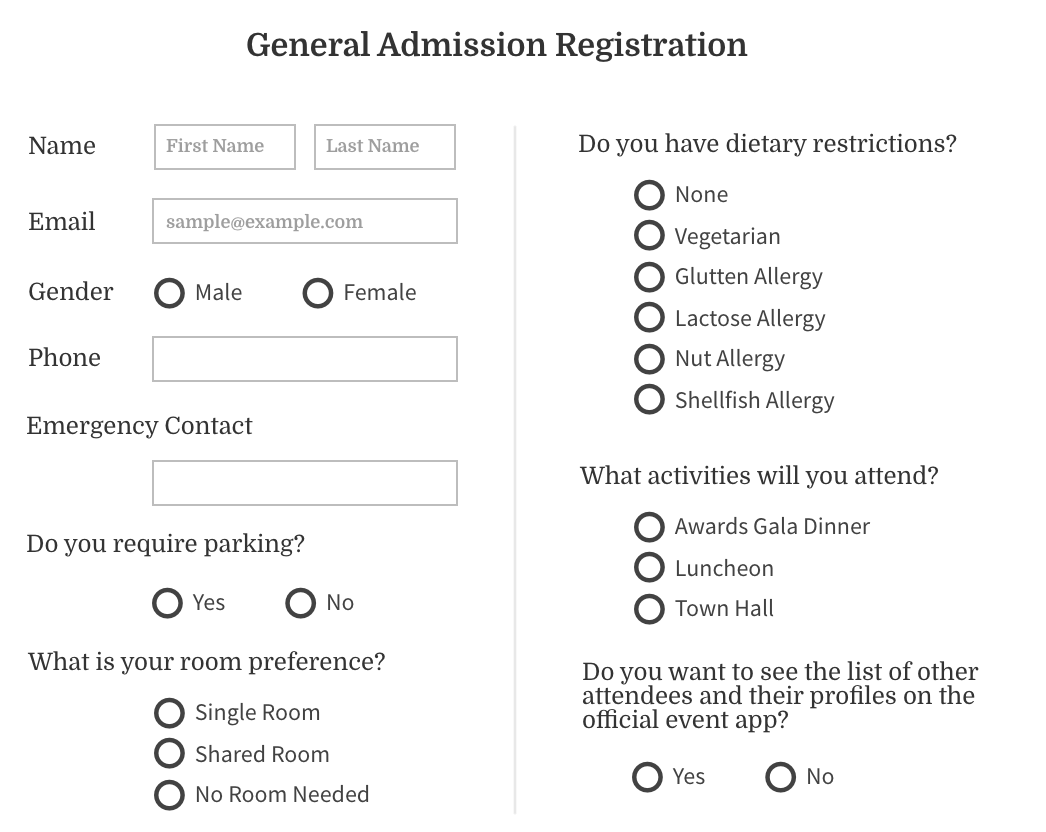
\includegraphics[scale=0.35]{slike/login_screen2.PNG} %veličina slike u odnosu na originalnu datoteku i pozicija slike
			\centering
			\caption{Primjer login screena (2)}
			\label{fig:promjene}
		\end{figure}
		
		Pri registraciji korisnik također mora odabrati jednu od navedenih uloga:
		\begin{packed_item}
			\item voditelj postaje
			\item istražitelj
			\item tragač
		\end{packed_item}
		
		\begin{figure}[H]
			
\includegraphics{slike/biranje_uloge.PNG} %veličina slike u odnosu na originalnu datoteku i pozicija slike
			\centering
			\caption{Primjer biranja uloge}
			\label{fig:promjene}
		\end{figure}
		
		U slučaju odabira uloge voditelja postaje, korisnik odabire dostupne postaje.
		Registracija korisnika potvrđuje se mailom, a u slučaju registracije za ulogu \textit{istraživača} ili \textit{voditelja postaje} potrebna je i dodatna potvrda od strane administratora.
		Registrirani korisnik može pregledati svoje osobne podatke.
		
		\textbf{Voditelj postaje} ima pregled svih članova postaje. Omogućeno mu je dodavanje novih tragača u postaju i uklanjanje dosadašnjih. Voditelj postaje je ujedno zadužen i za definiranje na koji su način tragači osposobljeni izvoditi pretraživanje. Mogući načini izvođenja pretrage su:
		
		\begin{packed_item}
			\item pješke
			\item dronom
			\item automobilom
			\item cross motorom
			\item brodom
			\item helikopterom
		\end{packed_item}
		
		Svaka metoda pruža različitu vidljivost i područje pokrivanja. Na primjer, zračno pretraživanje će obuhvatiti veće područje, ali neće pružiti toliko detalja kao što bi se dobilo pješačenjem.
		
		Još jedna bitna zadaća voditelja postaje je da alocira svoje tragače prema pristiglim zahtjevima od strane istražitelja. Voditelj šalje tragača na sudjelovanje u navedenoj akciju, a smije ga maknuti s akcije i ponovno učiniti raspoloživim isključivo ako je tragač završio sa svojim zadatkom u toj akciji.
		
	\begin{figure}[H]
			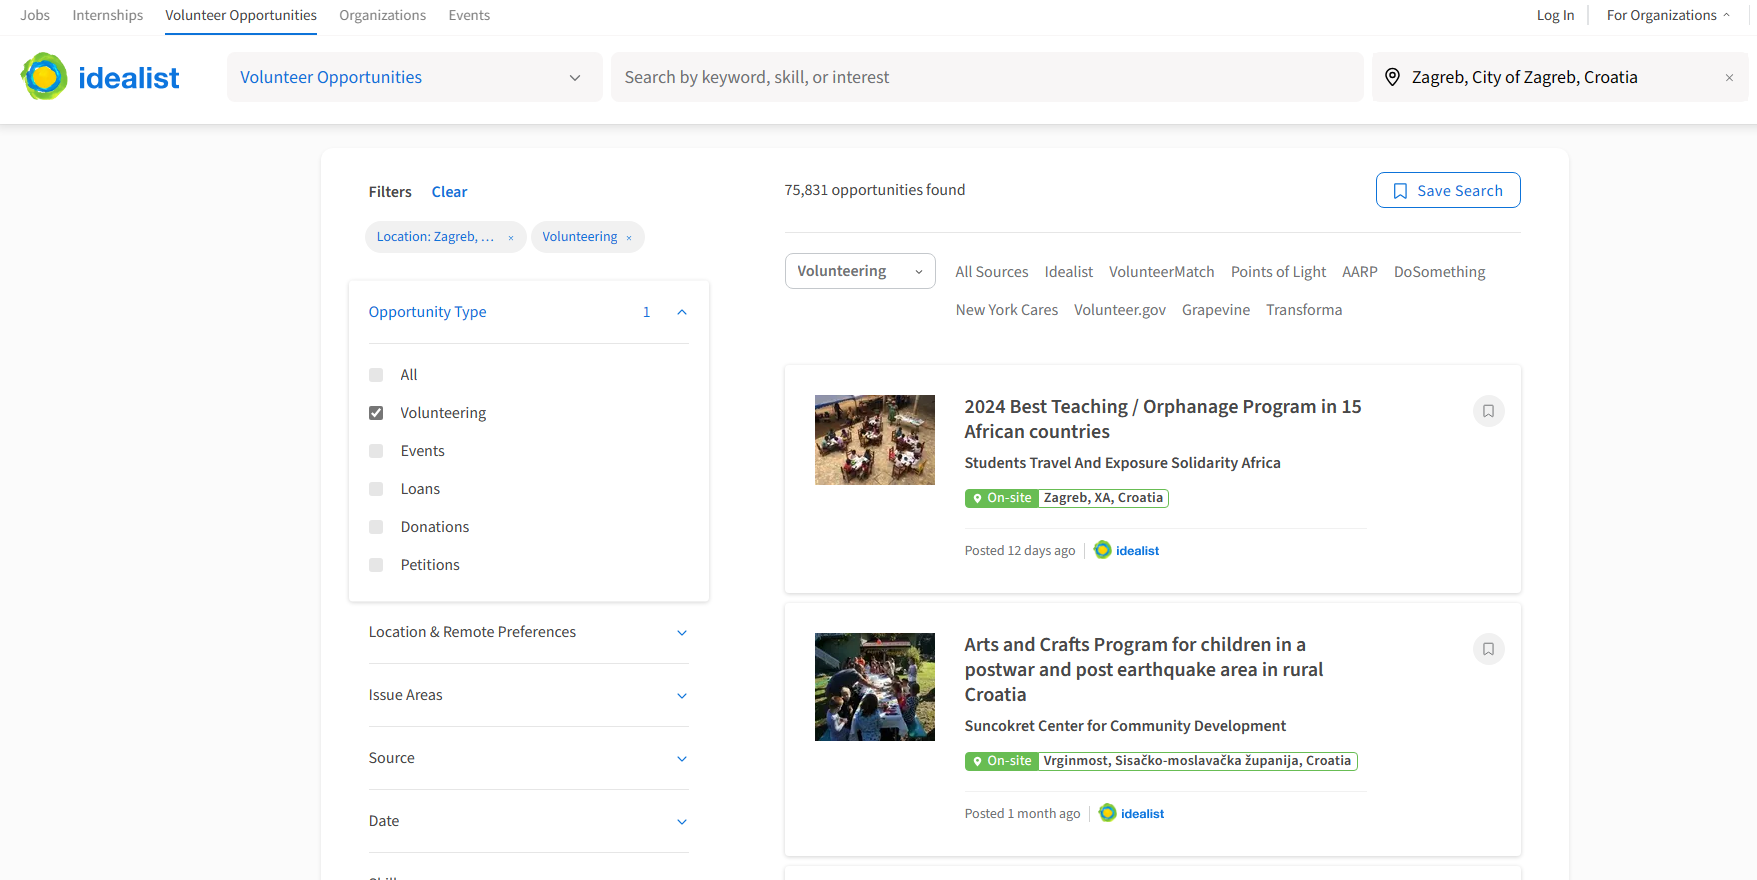
\includegraphics[scale=0.35]{slike/pr_biranje_akcije.PNG} %veličina slike u odnosu na originalnu datoteku i pozicija slike
			\centering
			\caption{Primjer biranja akcija}
			\label{fig:promjene}
		\end{figure}
		
		\begin{figure}[H]
			
\includegraphics[scale=0.35]{slike/pr_prihvacanje_akcije.PNG} %veličina slike u odnosu na originalnu datoteku i pozicija slike
			\centering
			\caption{Primjer prihvaćanja akcije}
			\label{fig:promjene}
		\end{figure}
		
		\textbf{Istraživač} je osoba koja ne pripada niti jednoj postaji, a njegova uloga je organizacija akcija pretraživanja i praćenja s detaljima o određenim vrstama, jedinkama ili staništima za proučavanje. Istraživač može stvoriti novu akciju sa svim potrebnim detaljima te poslati zahtjeve za tragačima  s opisom o potrebnim kvalifikacijama voditeljima različitih postaje. On ima pregled svih akcija koje je pokrenuo, kao i tragača koji sudjeluju u tim akcijama. Istraživač preko karte tragačima pojedinačno zadaje zadatke. Zadaci mogu tražiti prolazak određenom rutom i dolazak do određene lokacije te postavljanje kamere ili uređaja za praćenje. Svaki zadatak može imati i dodatan komentar od istraživača. Istraživač je taj koji po završetku zadatka označava da je tragač s njim završio.
		
		Glavni alat dostupan istraživaču je interaktivna karta. Njome se istraživaču prikazuju informacije o pozicijama životinja, tragača i postaja, a istraživač može izabrati da se za njenu izradu koristi neka od idućih informacija: 
		
		\begin{packed_item}
			\item povijesne pozicije svih praćenih životinja, filtrirano po vrsti ili pojedinačno po jedinki 
			\item trenutne pozicije praćenih životinja
			\item povijesne pozicije svih tragača na nekoj akciji, filtrirano po tipu prijevoza ili pojedinačno po tragaču 
			\item trenutne pozicije tragača aktivnih na akciji
		\end{packed_item}
		
		Informacije o povijesnim pozicijama se prikazuju preko toplinskih karata (engl. heatmap). Toplinske karte tragača su vizualizacija staza kojima su tragači putovali i načina kojim su se kretali, a služe kako bi istraživač mogao analizirati obrasce kretanja životinja i omiljena staništa.
		
		\begin{figure}[H]
			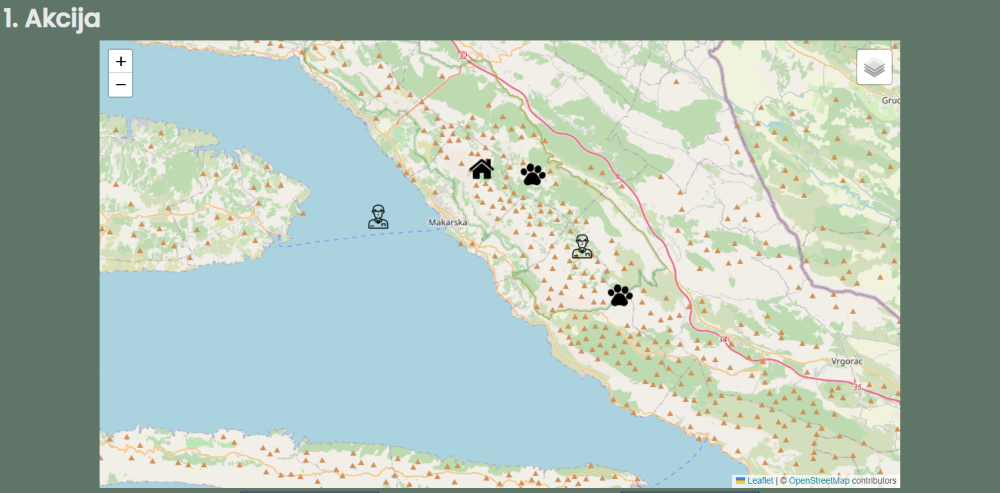
\includegraphics[scale=0.4]{slike/map_tracking.PNG} %veličina slike u odnosu na originalnu datoteku i pozicija slike
			\centering
			\caption{Primjer kartografskog prikaza (1)}
			\label{fig:promjene}
		\end{figure}
		
		\begin{figure}[H]
			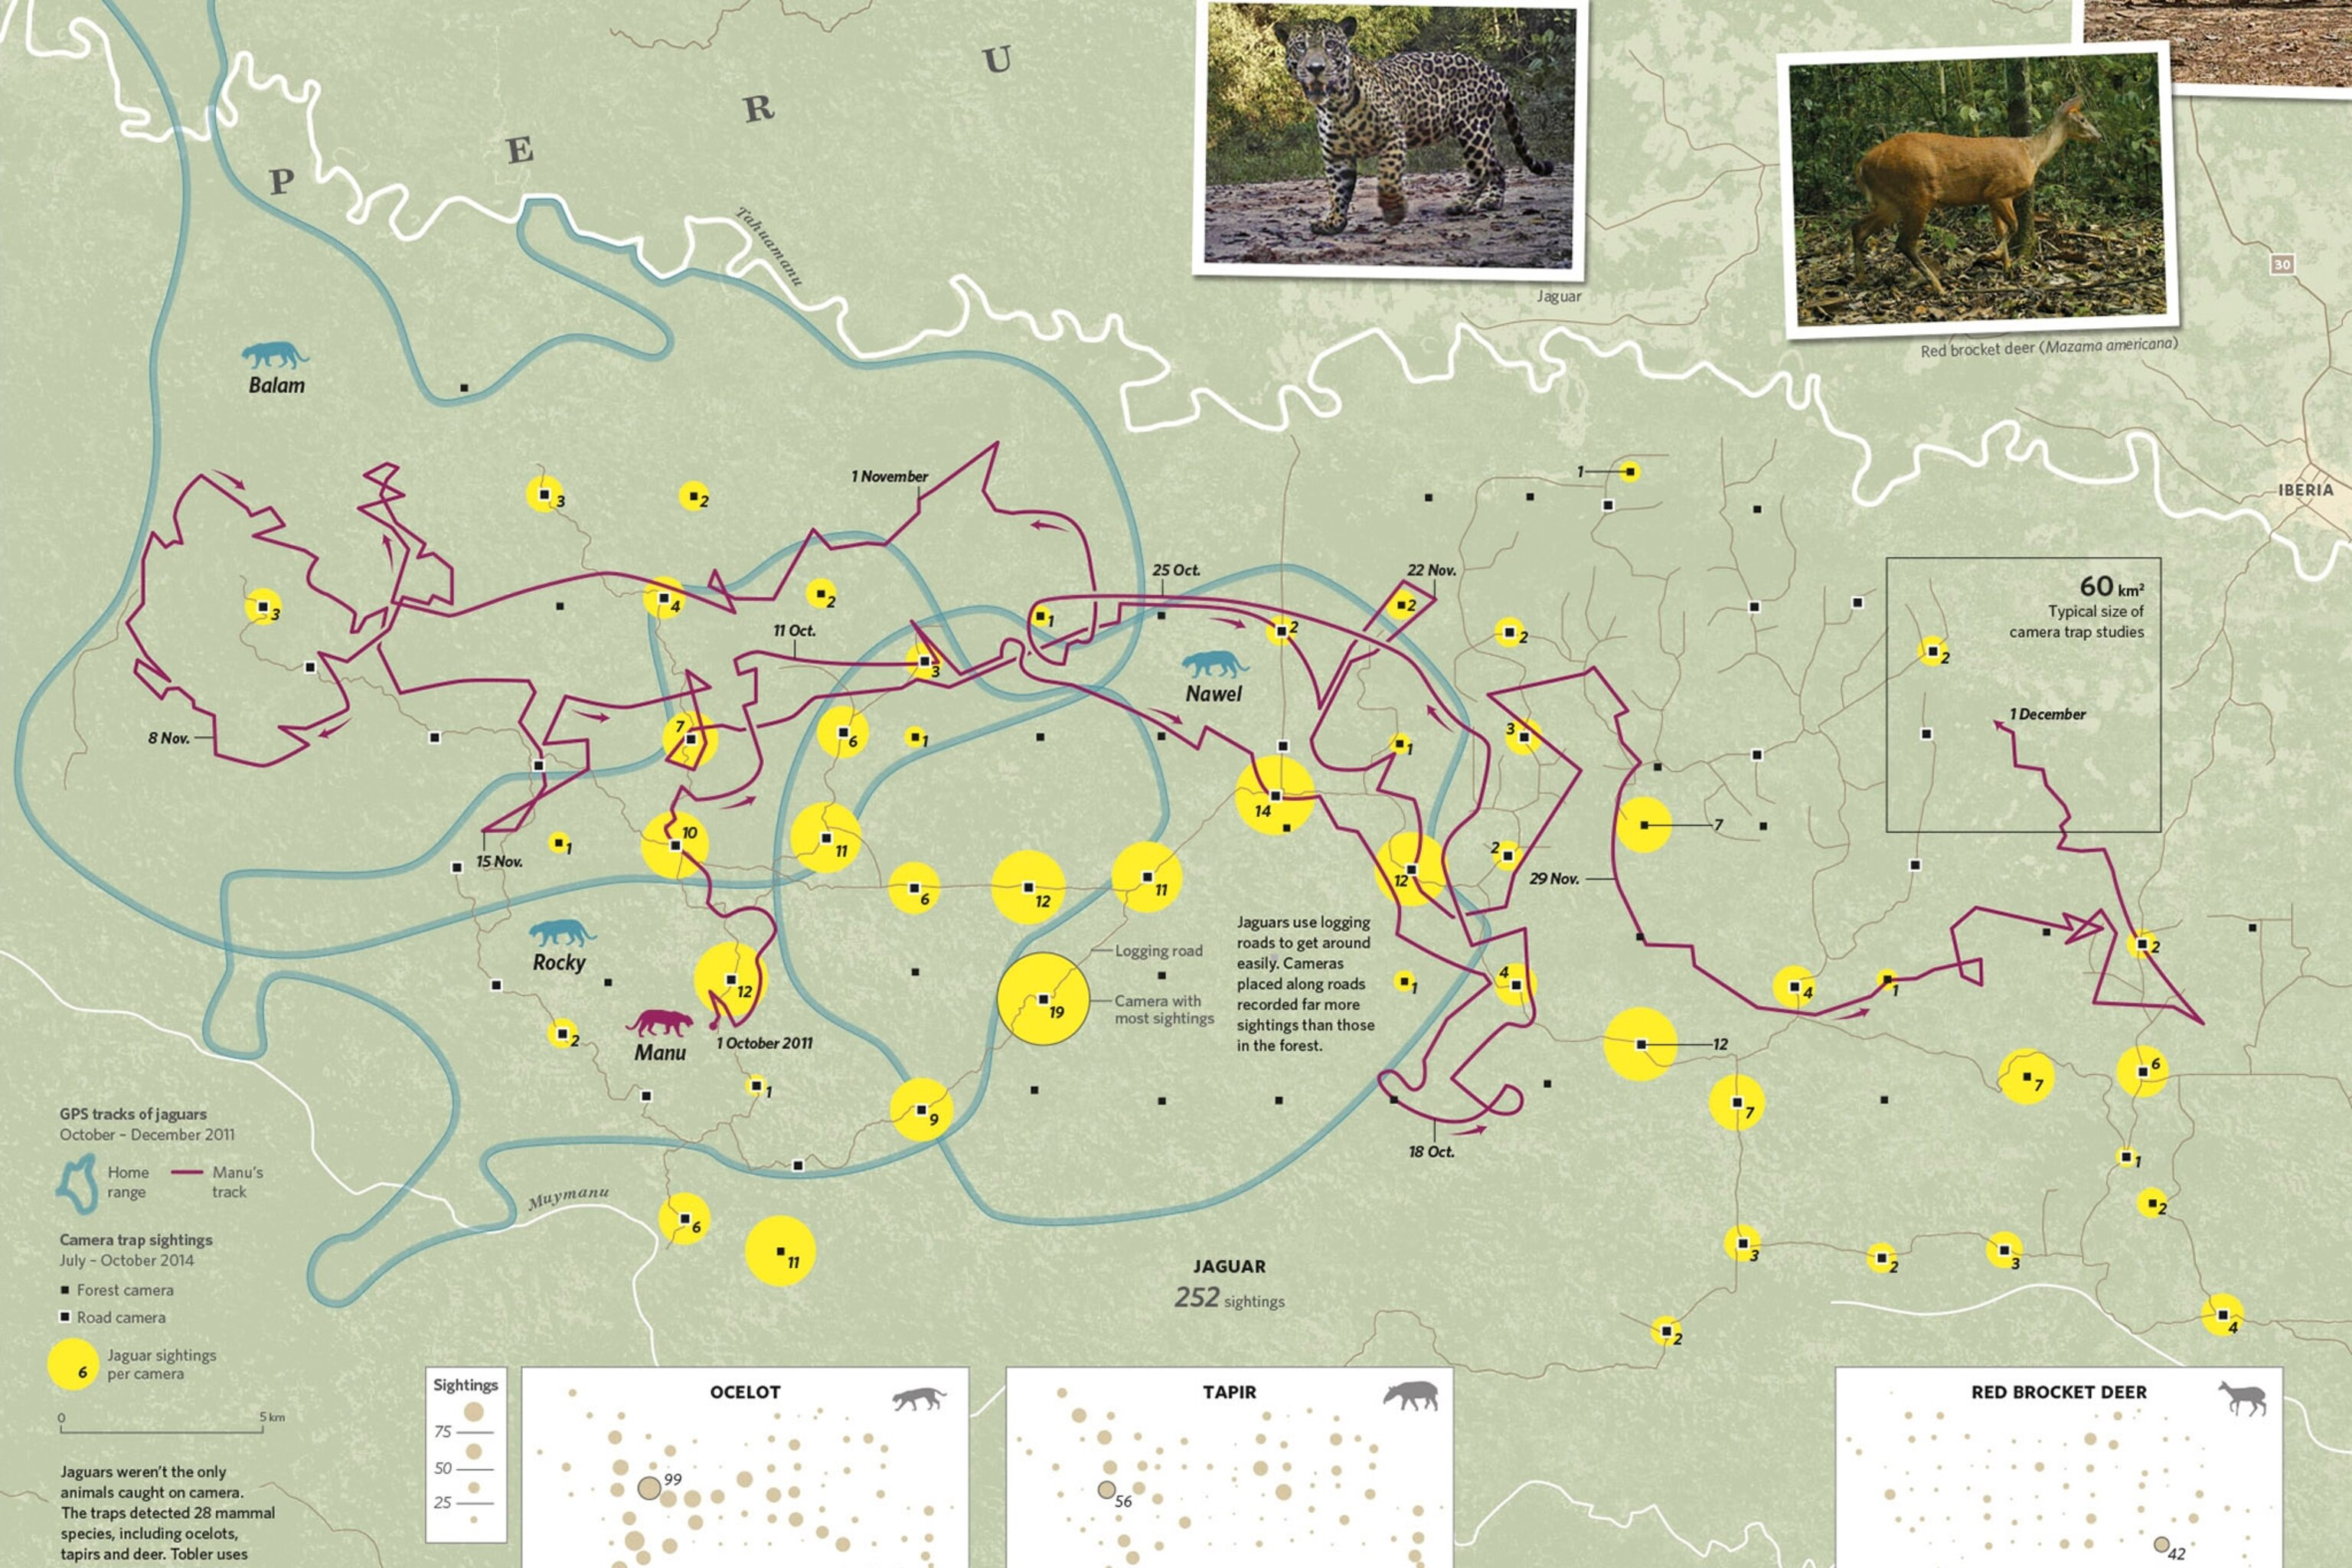
\includegraphics[scale=0.13]{slike/map_tracking2.PNG} %veličina slike u odnosu na originalnu datoteku i pozicija slike
			\centering
			\caption{Primjer kartografskog prikaza (2)}
			\label{fig:promjene}
		\end{figure}
		
		\textbf{Tragač} će nakon same kreacije korisničkog računa biti slobodan i ostati takav dok ga neki voditelj ne doda u svoju postaju. Time mu se otvara mogućnost sudjelovanja u akcijama. Za vrijeme neke akcije, tragaču se na karti prikazuju zadaci koje treba obaviti, trenutna pozicija ostalih tragača aktivnih na istoj akciji, te trenutna pozicija praćenih životinja. Praćene životinje na sebi imaju gps uređaj koji aplikaciji odašilje svoju poziciju. O
		praćenim životinjama se zapisuju povijesni podaci gdje se nalazila, naziv vrste, slika i opis. Tragač može praćenoj životinji tijekom akcije ostaviti komentar. Također, tragač i istraživač mogu na karti ostaviti komentar za ostale sudionike u akciji.		
		
		\textbf{Administrator} sustava ima najveće ovlasti. On ima pregled svih poslanih zahtjeva za registraciju u ulozi istraživača ili voditelja postaje koje on mora potvrditi ili odbiti. Administrator ima pristup bazi s popisom svih registriranih korisnika i njihovih osobnih podataka te ih može mijenjati. On ujedno može i mijenjati ulogu dodijeljenu korisniku.
\vspace{12pt}

		Iako naša aplikacija ima mnogo specifičnih značajki usmjerenih praćenju životinja te ostalih korisnika, možemo pronaći slične značajke i u nekim drugim aplikacijama koje se bave praćenjem i kontekstu prirode i istraživanja. Primjeri uključuju aplikacije kao što su:
		
		\begin{packed_item}
		
			\item \textbf{Wildme}\linebreak
			Wildme je organizacija koja razvija tehnologiju prepoznavanja uzoraka koja omogućuje automatsko prepoznavanje pojedinaca u divljini putem fotografija i drugih podataka. Ima seriju online platformi unutar \textbf{Wildbook} projekta usmjerena na analizu i praćenje životinja. Time omogućuje zoolozima i istraživačima praćenje lakše praćenje jedinki.
\vspace{12pt}
			
			\item \textbf{iNaturalist}\linebreak
			iNaturalist je stranica koja omogucuje korisnicima dijeljenje svojih opažanja divljih biljka i životinja. Koristi se za indetifikaciju vrsta te obilježavanje raznolikosti vrsta u prirodi.
\vspace{12pt}
			
			\item \textbf{Movebank}\linebreak
			Movebank je stranica za praćenje migracija životinja. Koristi se za pohranu i analiziranje podataka o kretanju životinja označene GPS uređajima
\vspace{12pt}
			
			\item \textbf{Panthera}\linebreak
			Pantera je organizacija posvećena očuvanju divljih mačaka. Njihovi projekti uključuju praćenje životinja te suradnje s lokalnim zajednicama.
			
		\end{packed_item}
		
        \begin{figure}[H]
			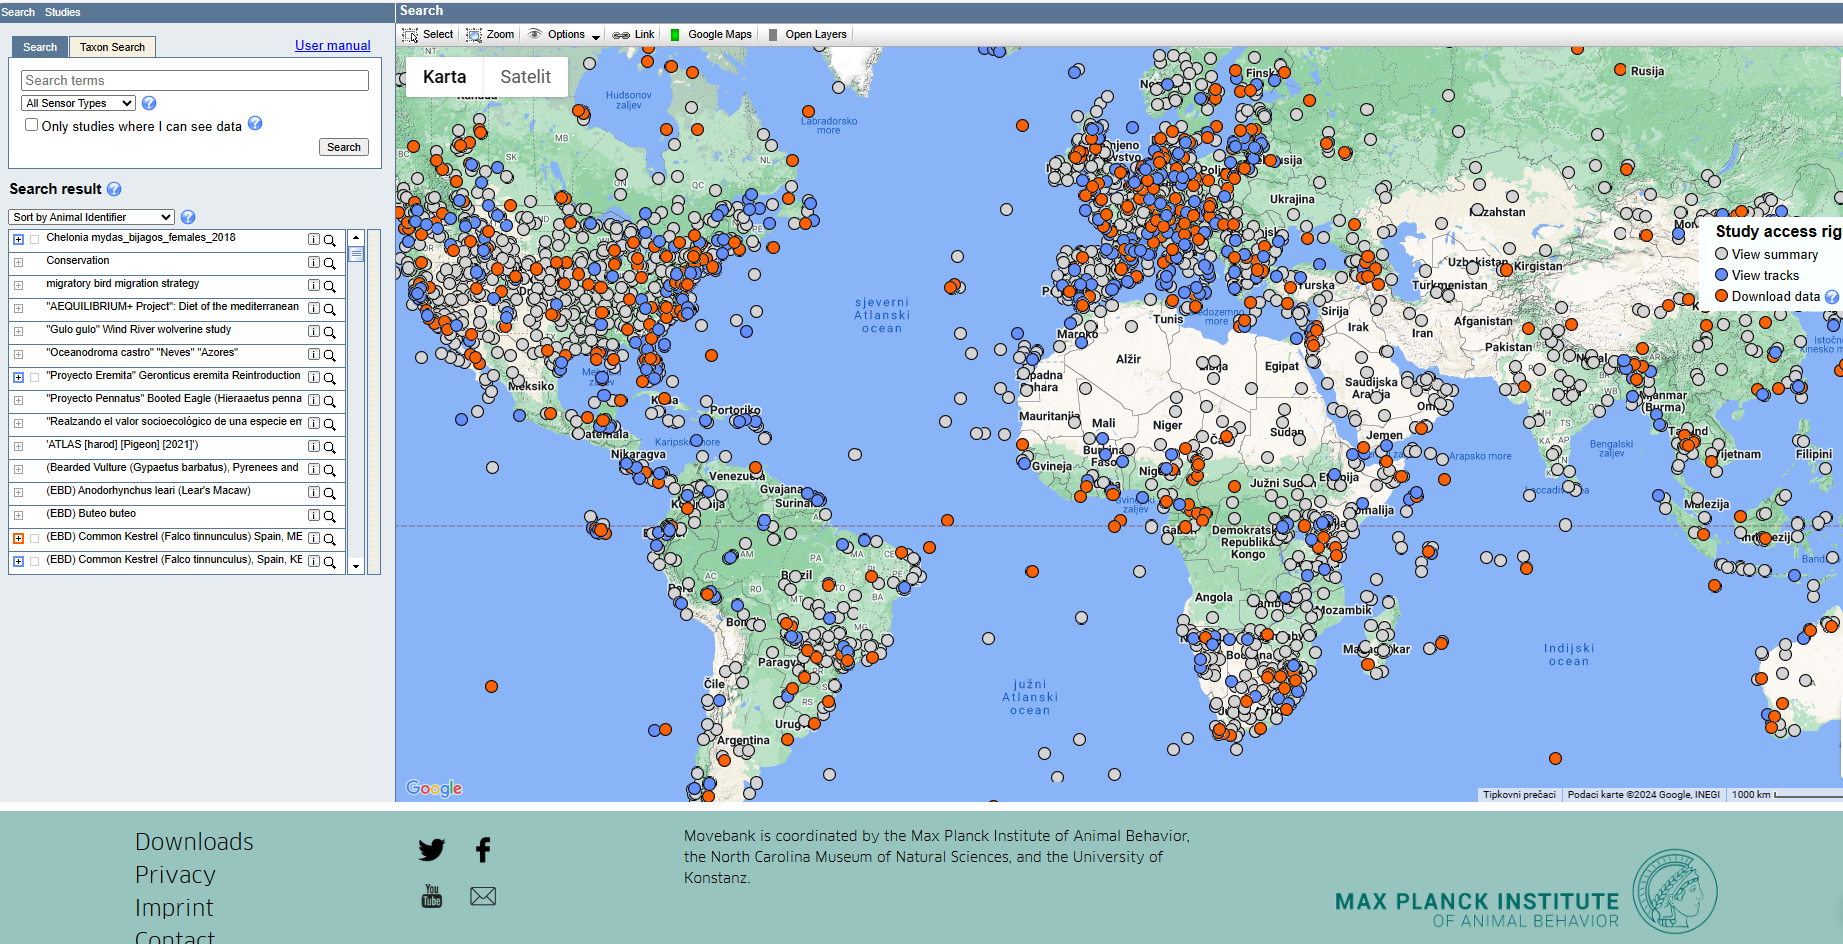
\includegraphics[scale=0.25]{slike/karta_movebank.PNG} %veličina slike u odnosu na originalnu datoteku i pozicija slike
			\centering
			\caption{Karta za praćenje životinja - Movebank}
			\label{fig:promjene}
		\end{figure}
		
		\begin{figure}[H]
		    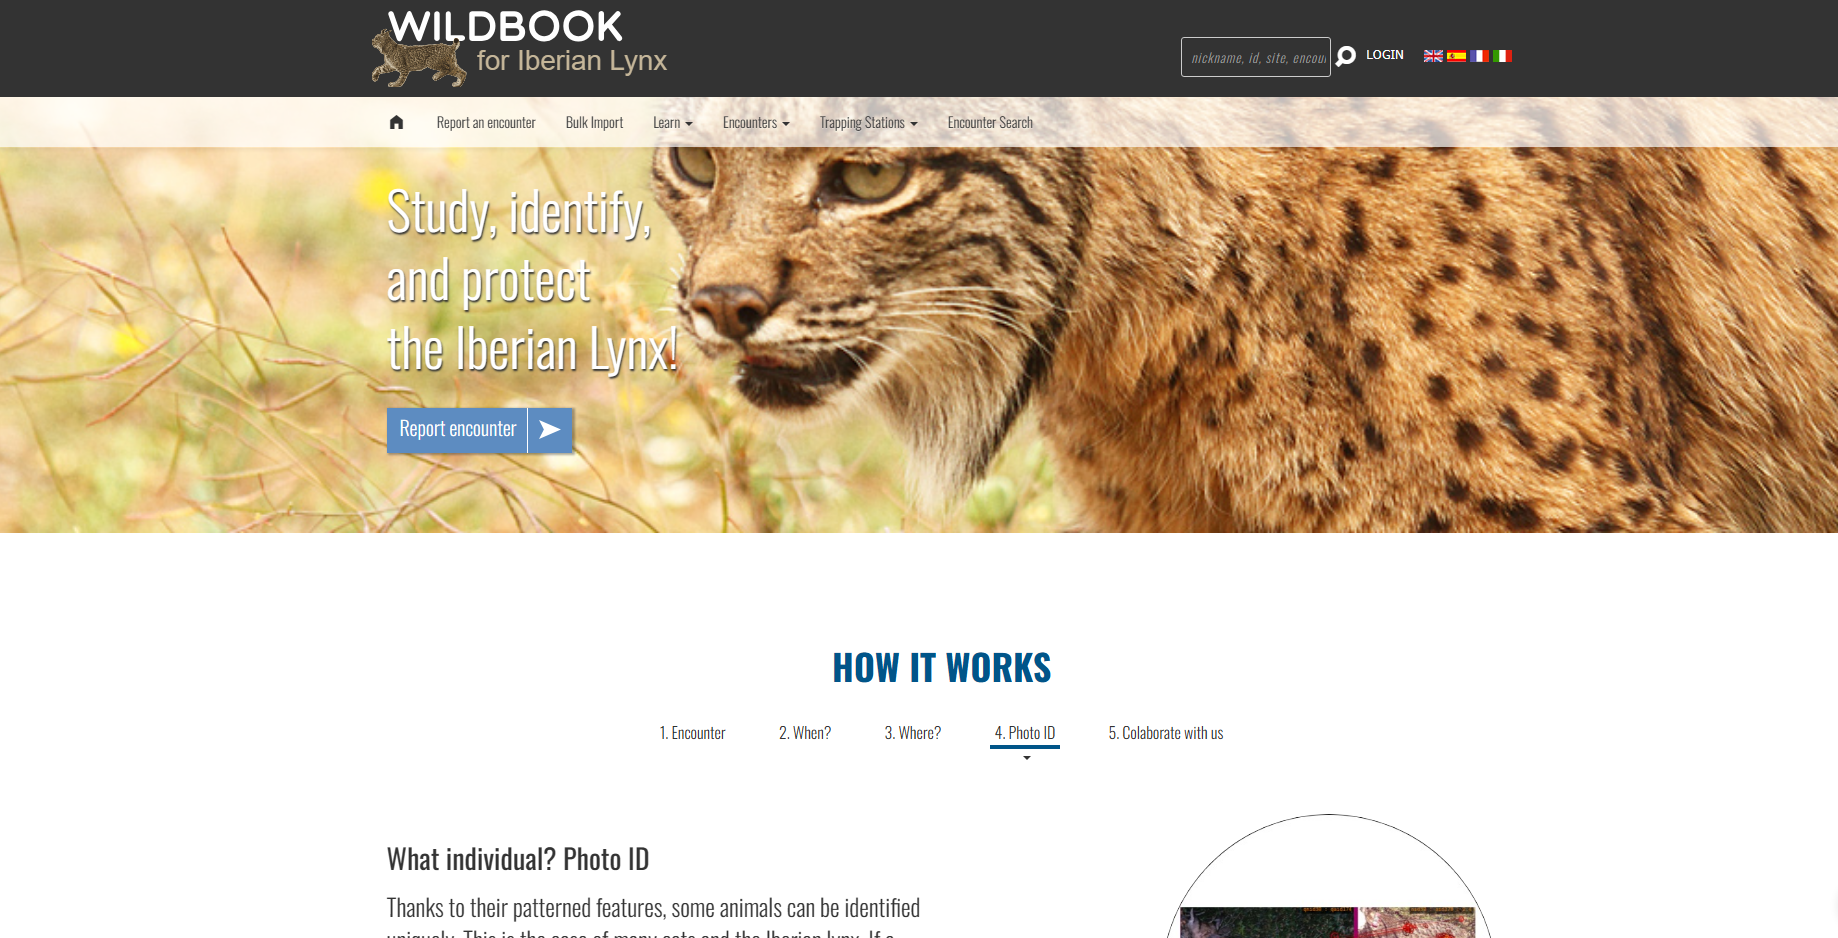
\includegraphics[scale=0.25]{slike/wildbook_ris.PNG} %veličina slike u odnosu na originalnu datoteku i pozicija slike
			\centering
			\caption{Wildbook za Pirenejskog risa}
			\label{fig:promjene}
		\end{figure}
		
		\begin{figure}[H]
			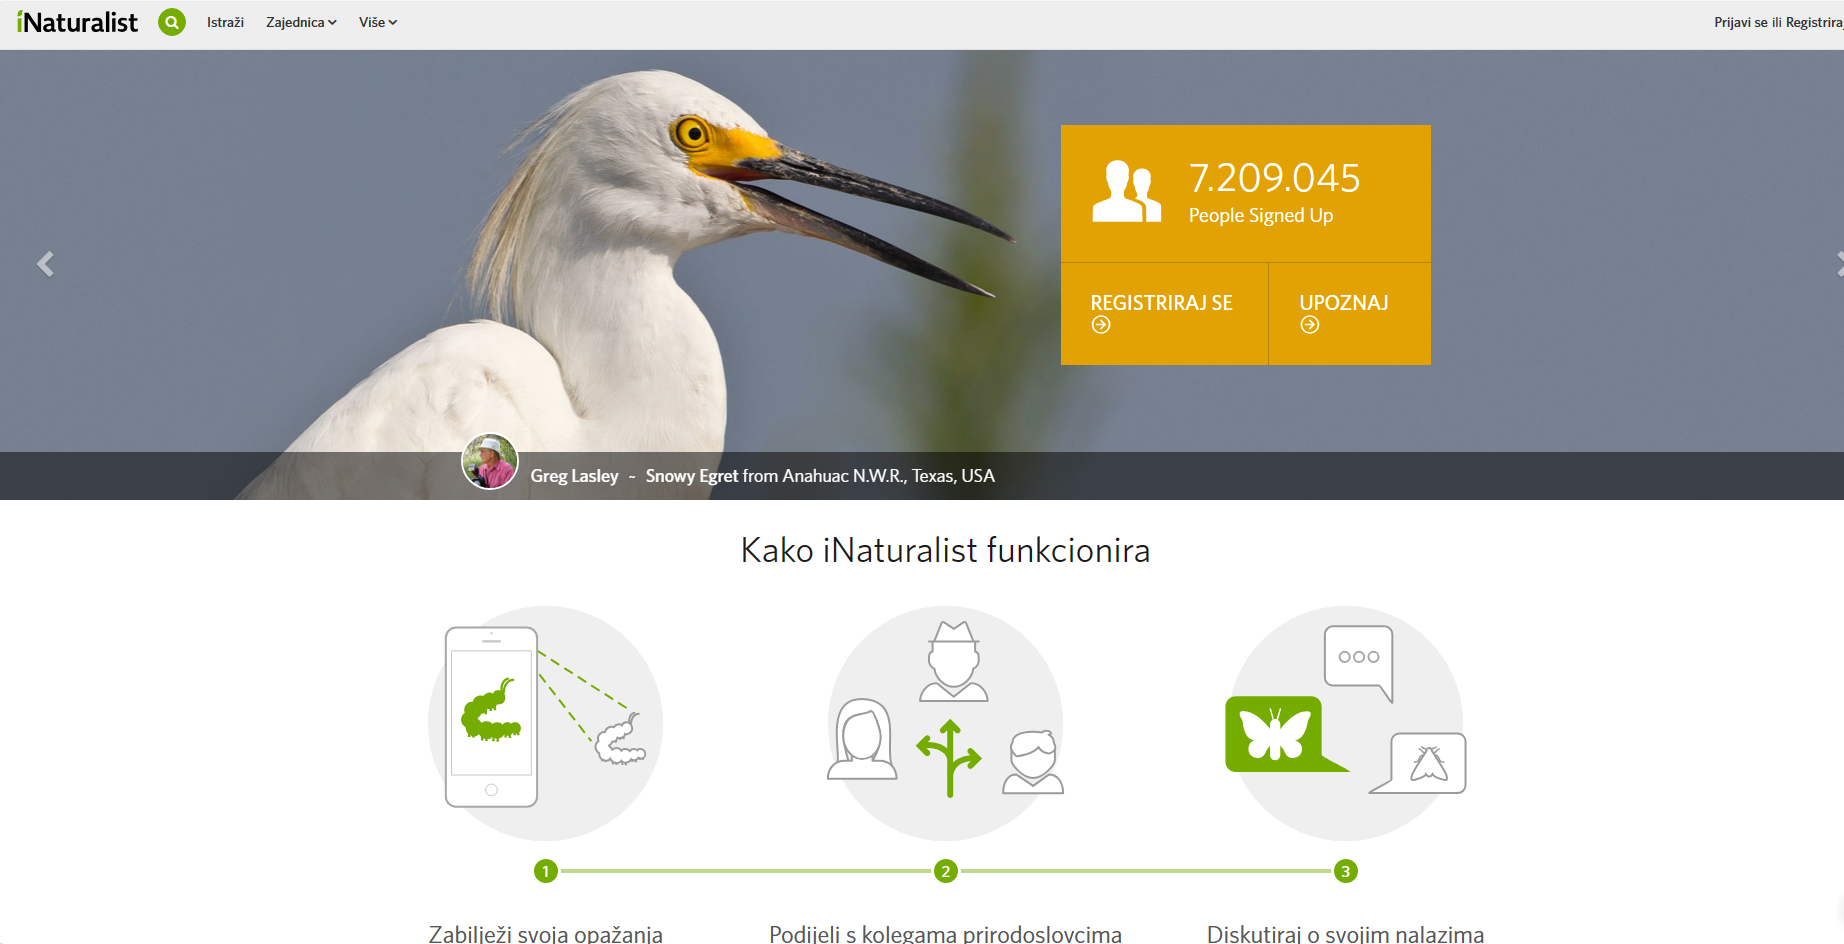
\includegraphics[scale=0.25]{slike/stranica_inaturalist.PNG} %veličina slike u odnosu na originalnu datoteku i pozicija slike
			\centering
			\caption{Stranica iNaturalist}
			\label{fig:promjene}
		\end{figure}